%!TEX root = main.tex
\setcounter{chapter}{5}
\setcounter{section}{4}
\setcounter{theorem}{0}
\setcounter{equation}{0}

\lectureheader{161}{Calculus I}{Fundamental theorem of calculus}{\textit{Thomas' Calculus} \thesection}

\begin{theorem}[Mean value theorem for integrals]
If $f$ is continuous on $[a,b]$, then there is a $c\in [a,b]$ so that
\begin{equation*}
f(c) = \frac{1}{b-a}\int_a^bf(x)\dee x.
\end{equation*}
\end{theorem}
\begin{proof}\,

\vspace{5.5in}
\end{proof}

\newpage

\begin{example}
Suppose that for time $t \in [a,b]$ (measured in seconds) the velocity of an object moving along the $s$-axis is $v(t)$ (measured in meters per second).
What does the accumulation function 
\begin{equation*}
f(t)=\int_a^t|v(u)|\dee u
\end{equation*}
represent, and what are its units?
What about the accumulation function
\begin{equation*}
F(t)=\int_a^tv(u)\dee u?
\end{equation*}
\end{example}

\newpage

\begin{theorem}[Fundamental theorem of calculus, part I]
If $f$ is continuous on $[a,b]$, then the function
\begin{equation*}
F(x)=\int_a^xf(t)\dee t
\end{equation*}
is an antiderivative for $f$ on $[a,b]$, i.e., 
\begin{equation*}
F'(x)=\frac{\dee}{\dee x}\int_a^xf(t)\dee t = f(x).
\end{equation*}
\end{theorem}

\begin{example}
Calculate $\frac{\dee y}{\dee x}$ for the following.
\begin{enumerate}[label=(\alph*)]
\item $y = \DS\int_a^x(t^3+1)\dee t$
\vfill
\item $y = \DS\int_x^53t\sin t\dee t$
\vfill
\newpage
\item $y = \DS\int_1^{x^2}\cos t\dee t$
\vfill
\item $y = \DS\int_{1+3x^2}^4\frac{\dee t}{2+t}$
\vfill
\end{enumerate}
\end{example}

\newpage

\begin{corollary}
If $f$ is continuous on $[a,b]$, then the unique solution to the initial value problem
\begin{align*}
y' &= f(x) \quad (a\le x\le b),\\
y(a)&=y_0
\end{align*}
is given by 
\begin{equation*}
y = y_0+\int_a^xf(t)\dee t.
\end{equation*}
\end{corollary}

\begin{theorem}[Fundamental theorem of calculus, part II]
If $f$ is continuous on $[a,b]$ and $F$ is any antiderivative for $f$ on $[a,b]$, then
\begin{equation*}
\int_a^bf(x)\dee x = F(x)\Big]_a^b = F(b)-F(a).
\end{equation*}
\end{theorem}

\begin{corollary}[Net change theorem]
If $f$ is continuously differentiable over $[a,b]$, then the net change in $f$ over $[a,b]$ 
\begin{equation*}
f(b)-f(a) = \int_a^bf'(x)\dee x.
\end{equation*}
\end{corollary}

\begin{example}
Evaluate $\DS\int_0^\pi\cos x\dee x$.
\end{example}



\newpage

\begin{example}
Evaluate the following
\begin{enumerate}[label=(\alph*)]
\item $\DS\int_{-\pi/4}^0\sec x\tan x\dee x$
\vfill
\item $\DS\int_1^4\left(\frac{3}{2}\sqrt x - \frac{4}{x^2}\right)\dee x$
\vfill
\end{enumerate}
\end{example}

\newpage



\begin{remark}
If $f$ is integrable over $[a,b]$, then the area enclosed by $y=f(x)$ and the $x$-axis is given by
\begin{equation*}
A = \int_a^b|f(x)|\dee x.
\end{equation*}
\end{remark}

\begin{example}
Determine the area of the region between the $x$-axis and the graph of $y=x^3-x^2-2x$ over $[-1,2]$.
\end{example}
\begin{flushright}
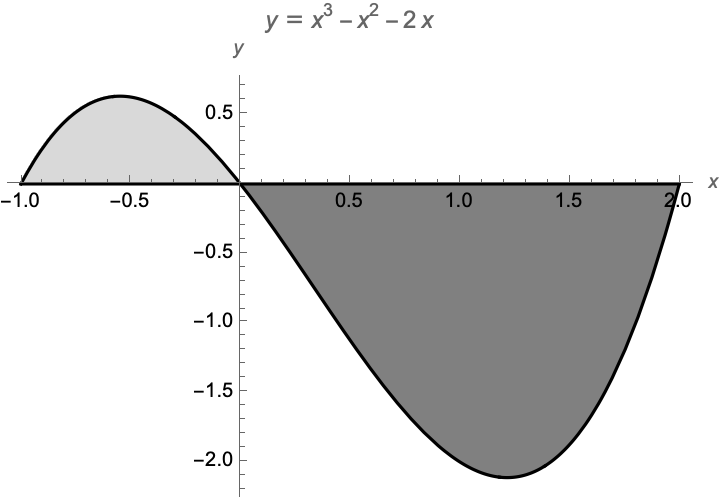
\includegraphics[width=3in]{img/area_example}
\end{flushright}

